\documentclass[12pt]{article}

\usepackage[utf8]{inputenc}
\usepackage[T1]{fontenc}
\usepackage{amsmath}
\usepackage{amssymb}
\usepackage{hyperref}
\usepackage{graphicx}

\graphicspath{{images/}}
\hypersetup{colorlinks=true, citecolor=blue}

\begin{document}

\title{Style Transfer from Non-Parallel Text by Cross-Alignment}
\author{}
\date{}
\maketitle

\section{Idea}
  The authors aim to perform style transfer on language using non-parallel corpora by separating content from style. They re-align the latent spaces to perform three tasks: sentiment modification, decipherment of word-substitution ciphers, and recovery of word order.

\section{Method}
  The authors' method involves learning an encoder that takes a sentence and its original style indicator as input, and maps it to a content representation devoid of style. This representation is then decoded by a style-dependent decoder.

  \subsection{Notation}
    $y \rightarrow$ latent style variable \\
    $z \rightarrow$ latent content variable \\
    $x \rightarrow$ data point generated from the conditional distribution $P(x|y,z)$ 

  \subsection{Formulation}
    There are two non-parallel corpora $X_1 = \{x_1^{(1)} ... x_1^{(n)} \}$, drawn from $p(x_1|y_1)$ and $X_2 = \{x_2^{(1)} ... x_2^{(n)} \}$, drawn from $p(x_2|y_2)$

    We want to estimate the style transferred distributions $p(x_1|x_2;y_1,y2)$ and $p(x_2|x_1;y_1,y2)$

    The authors propose a constraint that $x_1$ and $x_2$'s marginal distributions can only be recovered if for any different styles $y, y' \in Y$, distributions $p(x|y)$ and $p(x|y')$ are different, which is a fair assumption to make because if $p(x|y)$ = $p(x|y')$, then the style changes would be indiscernible. 
    
    They also prove that if the content $z$ is sampled from a centered isotropic distribution, the styles cannot be recovered from $x$, but in the case of $z$ being a more complex distribution like a Gaussian mixture, then the affine transformation that converts $y, z$ into $x$ can be recovered.

    The reconstruction loss is the same as the one used by an autoencoder
    \begin{eqnarray} \label{eq:reconstruction-loss}
      \mathcal{L}(\theta_E,\theta_G) 
        &=& \mathbb{E}_{x_1 \sim X_1}[-\log p_G(x_1|y_1,E(x_1, y_1))] + \nonumber \\
        & & \mathbb{E}_{x_2 \sim X_2}[-\log p_G(x_2|y_2,E(x_2, y_2))]
    \end{eqnarray}

  \subsection{Solution 1: Aligned Autoencoder} \label{aligned-autoencoder}
    Instead of the KL divergence loss, the authors propose aligning the distributions $P_E(z|x_1)$ and $P_E(z|x_2)$ where $E$ is the encoder function. This is done by training an adversarial discriminator to distinguish between the two distributions.

    The adversarial objective is expressed as below where $D(\cdot)$ predicts 0 if it predicts the source distribution to be $X_1$ and 1 if it predicts the source distribution to be $X_2$
    \begin{eqnarray} \label{eq:alignment-loss}
      \mathcal{L}_{adv}(\theta_E,\theta_D) 
        &=& \mathbb{E}_{x_1 \sim X_1}[-\log D(E(x_1,y_1))] + \nonumber \\
        & & \mathbb{E}_{x_2 \sim X_2}[-\log(1 - D(E(x_2,y_2)))]
    \end{eqnarray}

    The overall optimization objective combining equations \ref{eq:reconstruction-loss} and \ref{eq:alignment-loss} can be written as 
    \begin{equation*}
      \mathcal{L} = \operatorname*{min}_{E,G} \operatorname*{max}_{D} \mathcal{L} - \lambda \mathcal{L}_{adv}
    \end{equation*}

  
  \subsection{Solution 2: Cross-aligned Autoencoder}
    This is similar to the previous solution, but instead of trying to align $P_E(z|x_1)$ and $P_E(z|x_2)$ using an adversarial discriminator, two distinct adversarial discriminators are used to align a sequence of real and transferred generator hidden states. i.e. $D_1$ is used to align the distributions $G(y_1, z_1)$ and $G(y_1, z_2)$. Similarly, $D_2$ is used to align the distributions $G(y_2, z_2)$ and $G(y_2, z_1)$. These discriminators are trained with the objective of being unable to identify the content distributions $P(z_1)$ and $P(z_2)$

    Professor-forcing is used to train both of these discriminators. Professor forcing uses a discriminator to distinguish if the decoder hidden states are a result of training-time teacher forcing or test time scheduled sampling. This is a generalized version of simply using a final encoder state, as was the case in the Aligned Autoencoder solution (\ref{aligned-autoencoder}).

    The overall optimization objective combining equations \ref{eq:reconstruction-loss} and two discriminator versions of \ref{eq:alignment-loss} can be written as 
    \begin{equation*}
      \mathcal{L} = \operatorname*{min}_{E,G} \operatorname*{max}_{D} \mathcal{L} - \lambda (\mathcal{L}_{adv_1} + \mathcal{L}_{adv_2})
    \end{equation*}
    
    \subsection{Learning Process}
      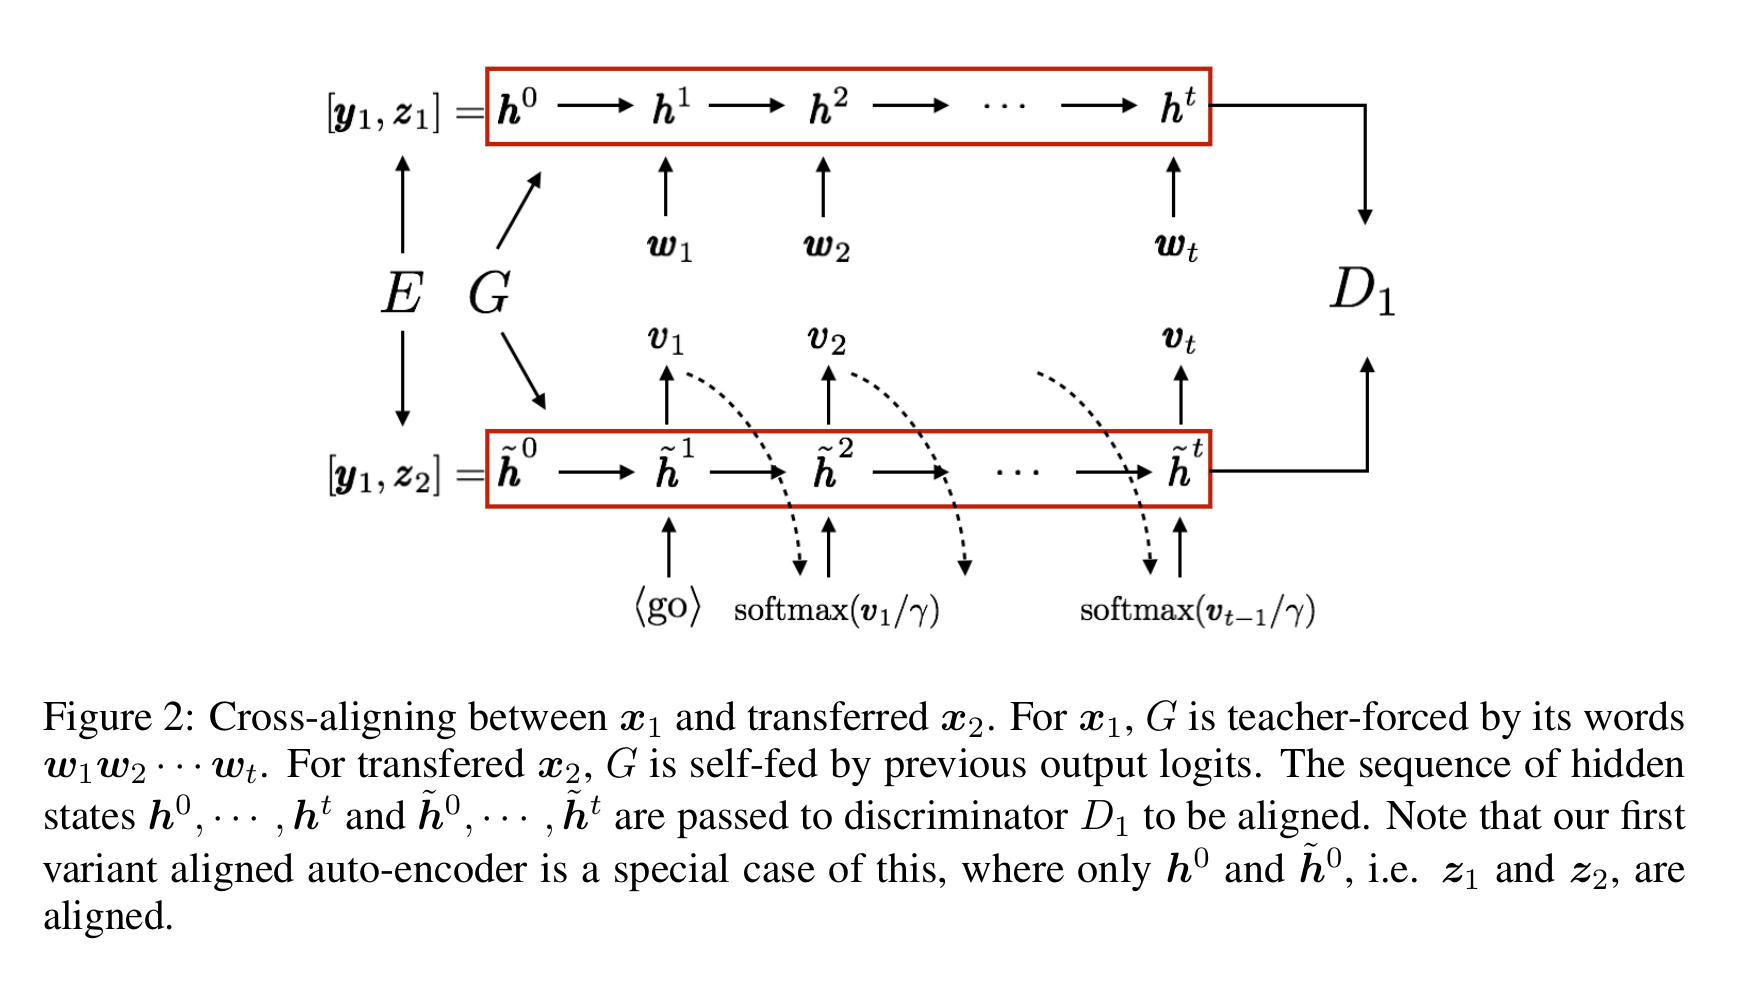
\includegraphics[width=\textwidth]{cross-alignment-training}
    
      \subsection{Experiment Setup}
      \begin{itemize}
        \item As opposed to the simple feed-forward classifier used for $D$ in the aligned autoencoder, $D_1$ and $D_2$ use convolutional nets for text classification \cite{kim2014convolutional}.
        \item They use Yelp reviews as the data set with rating $>3$ as positive and rating $<3$ as negative examples. Reviews with a sentence count $>10$ and sentences with a word count $>10$ are filtered out. Vocab size used is 10K.
        \item Style transfer is evaluated using a pre-trained classifier. \cite{kim2014convolutional}
        \item Content transfer was evaluation using human evaluations.
      \end{itemize}

\section{Observations}
  \begin{itemize}
    \item Despite the corpora being non-parallel, the content of both corpora is mostly homogenous.
    \item The authors cite the reason for not using VAEs for this task as the utility of having rich and unperturbed representations, which VAEs do not possess, because of the ELBO objective which forces the latent representation to be consistent with a prior distribution.
    \item The sentiment transfer model succeeds in retaining content 41.5\% of the time.
    \item The model described in \cite{hu2017toward} performed better in the sentiment style transfer task. The authors attribute this to the fact that their loss objective is directly parameterized by a sentiment classifier. Although the authors claim that the overall transfer quality is better, that metric is obtained from human evaluations and the difference is marginal.
    \item Amongst the different models, the cross-aligned autoencoder with one discriminator per style performs the best on all tasks.
  \end{itemize}

\bibliographystyle{unsrt}
\bibliography{style-transfer-from-non-parallel-text-by-cross-alignment}

\end{document}
